    \chapter{User guide}

\section{Registration}
\label{sec:registration}

\subsection{Step 1}
The reimbursement-tool is connected to the UZH-IFI LDAP server. This allows employees of the IFI department to use their existing login-credentials provided by the University of Zurich to login to the reimbursement-tool.\newline
After the initial login of a user its needed to pass thru a two-stepped registration process. On Figure \ref{fig:registration-step01} the user needs to input two values:
\begin{itemize}
    \item UZH personnel number is the employee number, written on the employment card. It is of the form \textit{01-123-456}. Enter the number without the leading 0 and hyphens; i.e. \textit{123456}.
    \item UZH phone number is the personnel phone number of the employee. Please enter it in the form \textit{0441234567}.
\end{itemize}


\begin{figure}[H]
    \centering
    \fbox{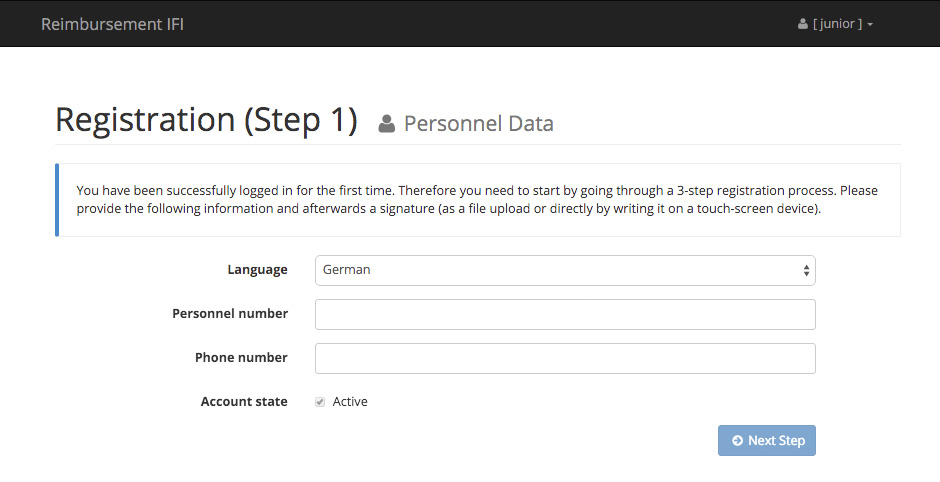
\includegraphics[width=0.80\textwidth]{registration-step01}}
    \caption{Registration step one: Capture personnel data}
    \label{fig:registration-step01}
\end{figure}

\subsection{Step 2}
On Figure \ref{fig:registration-step02} the user needs to add his handwritten signature either by uploading an image or capture it using a third party touchscreen device, like a smart phone. This signature is required to sign the generated Pdf document containing all \textit{Receipts}.

\begin{figure}[H]
    \centering
    \fbox{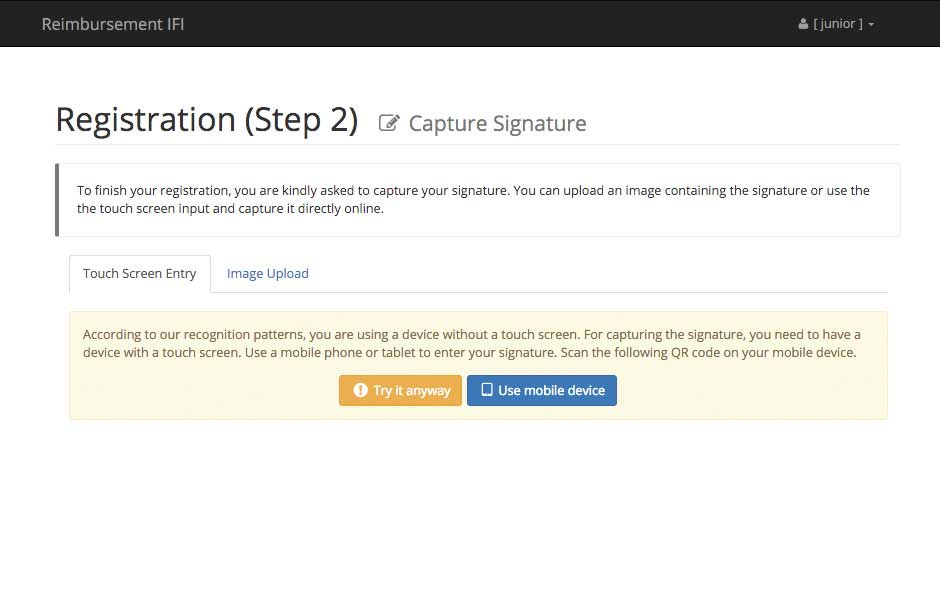
\includegraphics[width=0.80\textwidth]{registration-step02}}
    \caption{Registration step two: Capture signature}
    \label{fig:registration-step02}
\end{figure}

After completing the registration process, these captured information and signature can always be edited by navigation to the \textbf{Settings} on the navigation bar.
\clearpage

\section{Expenses}

An \textit{Expense} is an entity captured by an \textit{Employee}. Every \textit{Expense} is defined by an \textbf{accounting description} that will be visual in SAP. An \textit{Expense} consists of 1 to 15 \textit{Receipts}.

The \textit{Employee} has to create an \textit{Expense}, add \textit{Receipts} to it and assign it to his \textit{Manager}. The \textit{Manager} will check the \textit{Expense} for correctness, add the corresponding projects and assign it to the \textit{Finance administration} if the \textit{Expense} is correct. For a detailed description of the process refer to section \ref{sec:process}.

\subsection{Create expense}

To create an \textit{Expense}, the user needs to navigate to the \textbf{Dashboard} and click on the button \textbf{Create new Expense}. A modal-window will appear to enter an SAP description.\newline Once the \textit{SAP description} is entered correctly and the user clicked \textbf{Next} an empty \textit{Expense} will be created. The user can start with adding \textit{Receipts} (Figure \ref{fig:expensesitems-overview}).

\begin{figure}[H]
    \centering
    \fbox{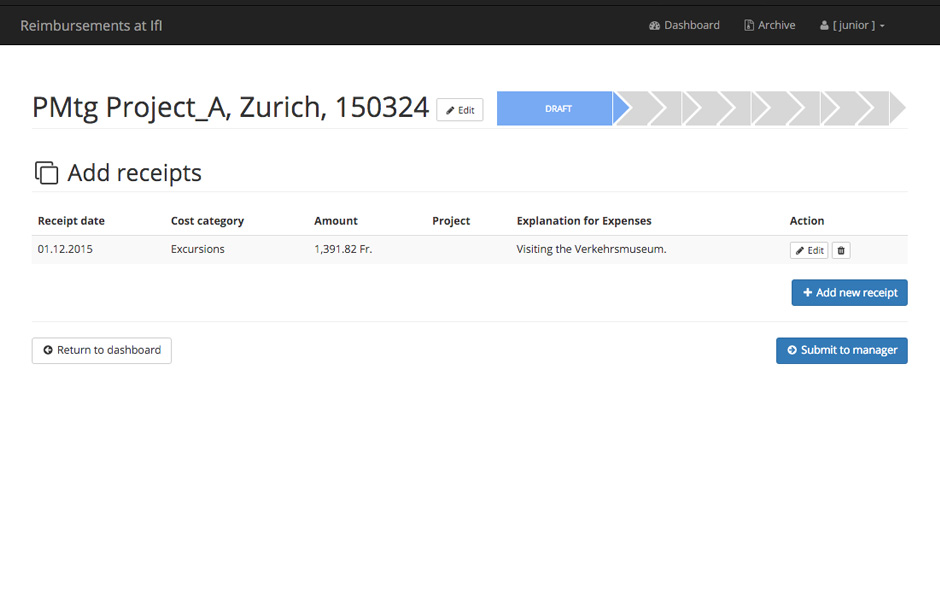
\includegraphics[width=0.80\textwidth]{expensesItems-overview}}
    \caption{Expense-View: Overview}
    \label{fig:expensesitems-overview}
\end{figure}

On the top left-hand side the \textit{SAP description} is added. The small button on the right can be used for editing. On the top right-hand side the current process step and the unprocessed steps of the \textit{Expense} are visualized. This process bar always indicates the state the \textit{Expense} is currently at.\newline
Further the user can add, edit and remove \textit{Receipts}. To add a new \textit{Receipt} the user needs to click on the button \textbf{Add new Receipt}. See Section \ref{sec:addreceipt} for details.\newline
Existing \textit{Receipts} can be edited and removed by clicking on the respective buttons at the Receipts-list.


\subsection{Add receipt}
\label{sec:addreceipt}
By adding a new \textit{Receipt} or editing an existing one, the user needs to fill out the following mandatory information:
\begin{itemize}
    \item \textbf{Receipt date} will further be used to calculate the correct exchange rate if a foreign currency is selected.
    \item \textbf{Cost category} selected based on a pre-defined list of available cost categories.
    \item Original and calculated amount based on the exchange rate.
    \item The \textbf{project assignment} is added by a user with role \textit{Manager} or \textit{Deputy manager}.
    \item A short \textbf{explanation} that describes the purpose of the \textit{Receipt}.
    \item \textbf{Receipt attachment} used for verification purpose of the entered \textit{Receipt} data.
\end{itemize}

See Figure \ref{fig:expenses-add01} for details.


\begin{figure}[H]
    \centering
    \fbox{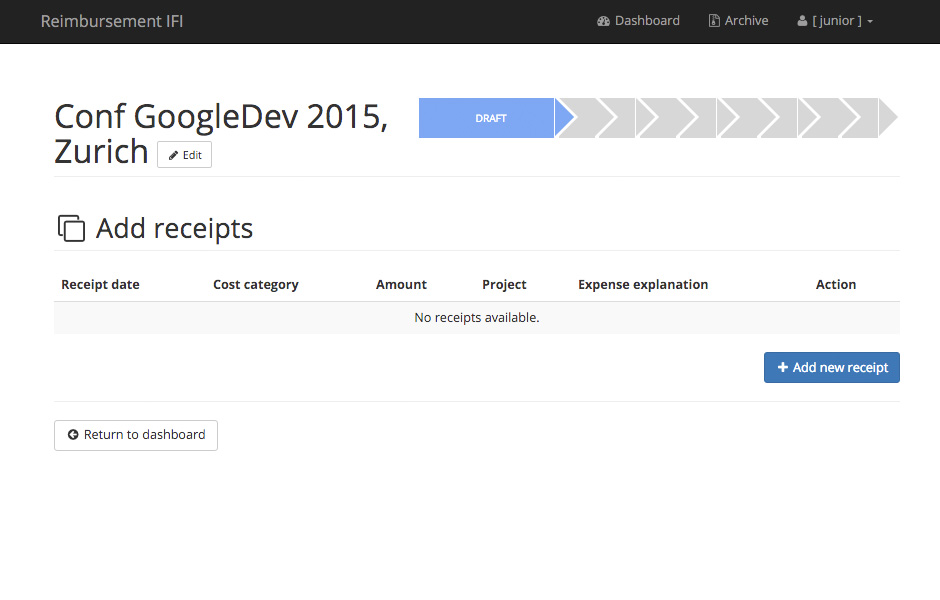
\includegraphics[width=0.80\textwidth]{expenses-add01}}
    \caption{Expense: Add new receipt}
    \label{fig:expenses-add01}
\end{figure}

\subsection{Assign expense to manager}
If all \textit{Receipts} are captured, the \textit{Expense} will be assigned to the \textit{Manager} in charge. Once the assignment is processed, the \textit{Expense} cannot be edited by the user anymore. To assign an \textit{Expense} to the \textit{Manager}, click on the \textbf{Submit to Manager} button.

\subsection{States}
\label{sec:states}
Every \textit{Expense} is always in one of the following states during the process:

\begin{itemize}
    \item \textbf{DRAFT} state occurs if the \textit{Expense} is created and yet has not been assigned to a \textit{Manager}.
    \item \textbf{ASSIGNED} state occurs if a \textit{Manager} or \textit{Deputy manager} has assigned the \textit{Expense} to him.
    \item \textbf{REJECTED} state occurs if the created \textit{Expense} is not accepted by the \textit{Manager}, \textit{Deputy manager} or \textit{Finance administrator}. In \textbf{REJECTED} status the \textit{Expense} will be reassigned to the user who created it.
    \item \textbf{SIGNED} state occurs if the \textit{Expense} has been signed by all three instances; \textit{Employee}, \textit{Manager} or \textit{Deputy manager} and \textit{Finance administrator}
    \item \textbf{PRINTED} state occurs if the \textit{Expense} and all its \textit{Receipts} are successfully converted into a digital document.
\end{itemize}

\subsection{Digital signature}
tbd

\section{User}

Every user that exists in the LDAP of the University of Zurich is capable to login to the system. He can use the same user name and password that he uses for the other University of Zurich services for login. See Section \ref{sec:registration} for more details.

There exists different roles for users to login to the system. A user is allowed to have exactly one role out of the four defined. The roles are provided and synchronized with the LDAP-Server of the University of Zurich. The following roles exist in the system:

\begin{itemize}
    \item \textbf{Employee} are authorized to create and edit \textit{Expenses} that they created. However, an \textit{Expense} cannot be edited once it has been assigned to a \textit{Manager}.
    
    \item \textbf{Manager} are authorized to reject, accept and edit \textit{Expenses}. A \textit{Manager} is also capable of creating \textit{Expenses} and editing them until it has been assigned.
    
    \item \textbf{Deputy manager} has the same authorizations as the \textit{Manager}. If a \textit{Manager} is outreach his assignments will be forwarded to the \textit{Deputy manager}. There exist multiple \textit{Deputy manager}.
    
    \item \textbf{Finance administrator} is authorized to reject, accept and edit \textit{Expenses} once they have been accepted by a \textit{Manager} or \textit{Deputy managers}. Furthermore they can manage the available cost categories.
    
    \item \textbf{Head of institute} has the same authorizations as the \textit{Manager}. In contrast to the \textbf{Deputy manager} there exists only one \textit{Head of institute}.
\end{itemize}

\section{Guest view}
The guest view allows users to retrieve \textit{Expenses} without the need of valid login-credentials for the reimbursement-tool. They can open the guest view using a special URL, provided on every printed \textit{Expense} document. The URL is located on the second page in form of a QR-Code and an URL. So that the user can either scan the QR-Code or typewrite the URL in a browser window and he'll get access to the respective \textit{Expense}.


\section{Process}
\label{sec:process}
As described in \ref{sec:states} an \textit{Expense} is always in one specific state. The entire process implemented in the system is shown in Figure \ref{fig:process-diagram}. The process is visualized using the BPML. Four lanes point out the available user roles. The process starts in the first lane; an \textit{Expense} is created, \textit{Receipts} are added and it is forwarded to the next higher instance for verification. After verifications by the \textit{Manager} or \textit{Deputy manager} and \textit{Finance administration} are successful, the user, \textit{Manager} and the \textit{Finance administration} needs to sign the document. If all users signed the document, it is ready to be printed by the user who created the \textit{Expense}.

\begin{figure}[H]
    \centering
    \fbox{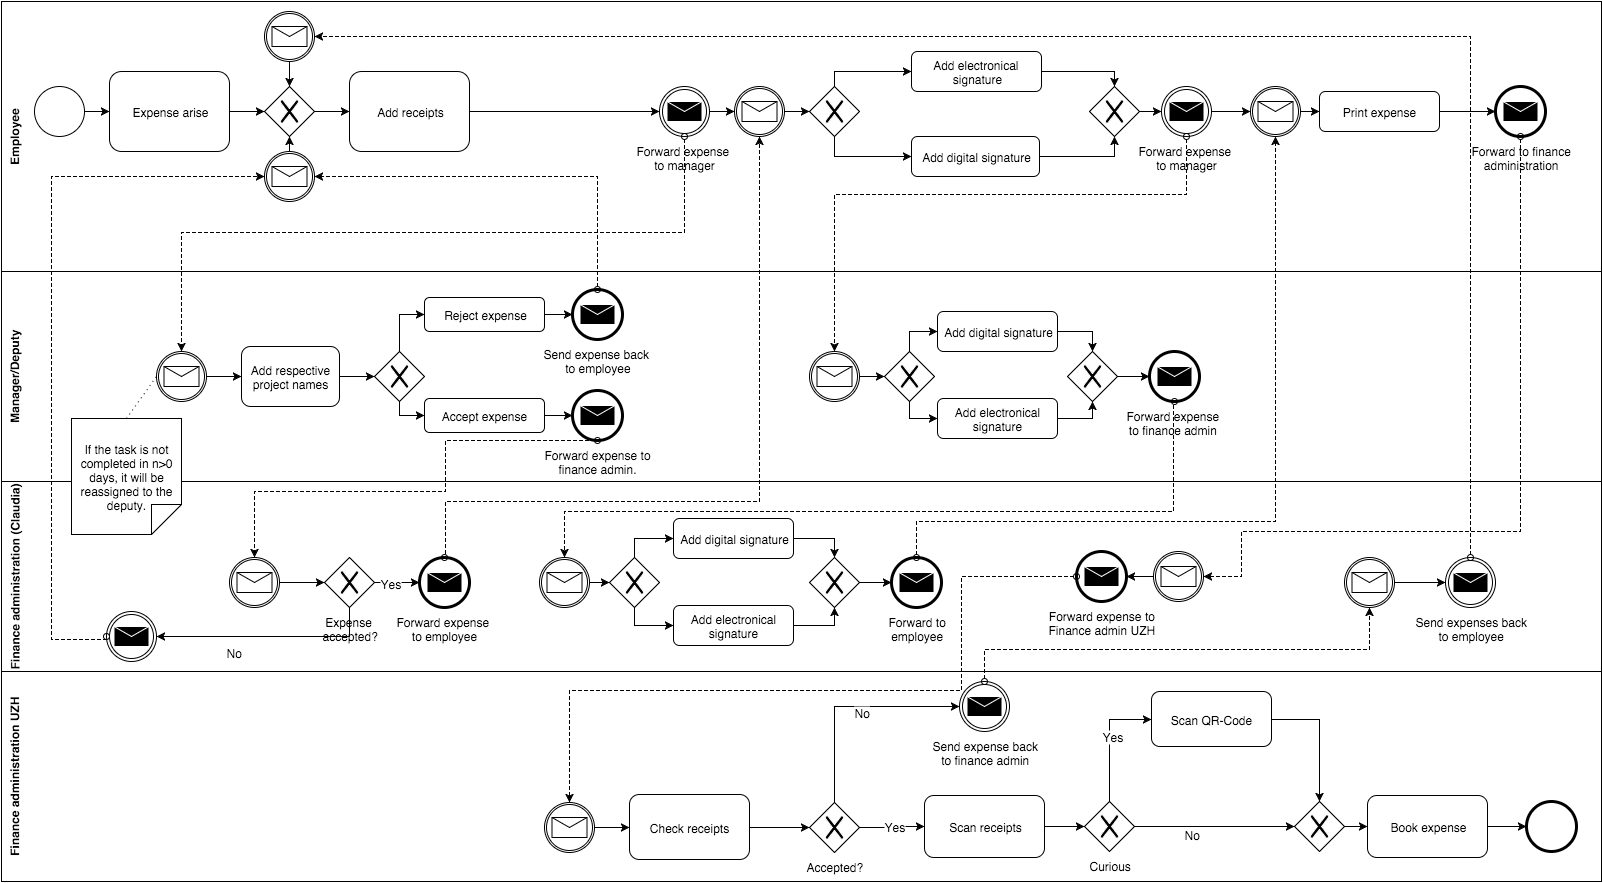
\includegraphics[width=0.80\textwidth]{process-diagram}}
    \caption{Expense: Workflow process}
    \label{fig:process-diagram}
\end{figure}
